%%%%%%%%%%%%%%%%%%%%%%%%%%%%%%%%%
% 6CCS3PRJ Final Year Individual Project Report
% ruihan.ji@kcl.ac.uk
%%%%%%%%%%%%%%%%%%%%%%%%%%%%%%%%%
\documentclass[11pt]{informatics-report}
\usepackage{color}
\usepackage{amsmath}
\usepackage[square,sort,comma,numbers]{natbib} %References
%%%%%%%%%%%%%%%%%%%%%%%%%%%%%%%%%
% Front Matter - project title, name, supervisor name and date
%%%%%%%%%%%%%%%%%%%%%%%%%%%%%%%%%
\title{6CCS3PRJ Final Year\\\vspace{0.2cm}Individual Project Report Title}
\author{Rui Han Ji Chen}
\studentID{K20027110}
\supervisor{Christopher Hampson}

\date{\today}

\abstractFile{FrontMatter/abstract.tex}
\ackFile{FrontMatter/acknowledgements.tex} %Remove line if you do not want acknowledgements

\begin{document}
\createFrontMatter
\onehalfspacing
\tableofcontents
\doublespacing

%%%%%%%%%%%%%%%%%%%%%%%%%%%%%%%%%
% Report Content
%%%%%%%%%%%%%%%%%%%%%%%%%%%%%%%%%
% You can write each chapter directly here or in a separate .tex file and use the include command.

\chapter{Introduction}


The Nucleic acid sequence is the set of characters that biologists use to represent the order of the nuclearbase (base) 
of DNA or RNA, the four letters used to represent are A, C, G and T (representing adenine, cytosine, guanine and 
thymine), in case of RNA, U (Uracil) would replace T. 

Every base sequence has its complementary as well as the characters, the letters are paired as A for T and C for G, so 
for example, the complementary sequence of ``ATCG'' would be ``TAGC''. This is essentially a stringology research, 
analyzing the sequence of the genetic code is important for the bioinformatics as this can be used to understand why
some living thing functions that way and also compare the sequence alignment to highlight the relationship between
different sequences. 
 
\section{Motivation}

After this long period of Covid pandemic, I understood how biology has such an impactful influence to our life, but at 
the same time I also noticed the benefits that computing can bring to traditional biology, eventhough there are already
algorithms that can solve the problem fair easily, however, I will focus my research on a more specific topic. The 
efficiency when calculating the sequence analysis can be resolved by better algorithm designs, as programmers, we 
can provide a better environment for other scientific researches. 

\section{Project aims}

The main objective of the project would be the deep research on Longest Common Subsequence problem which matches with
the concept of sequence alignment in biology, being a NP-Complete problem also aligns with the Computer Science theme. 
To go further with the idea of more efficiency, I want to compare different algorithms with some other s to see the 
differences in different dimensions (Speed would be one dimension as well as space). I will research and explain
the background logic of different kind of algorithms and also build my own one and also compare it with other ones.

The other objective would be the idea of building an algorithm application that can be used for a real-life scenario,
performing different experiments and functionalities, so for biologists who are not that familiar with computing can 
use the program or even build a similar one by just reading this project. 


\section{Report Structure}

The report will be started with a bit of background information about the concept of NP and NP-Completeness, as well
as understanding what is the Longest Common Subsequence problem and how its importance in biological researches by 
reviewing real life examples.

The next part would begin with understanding different kind of algorithms to solve LCS problems and compare them, this
section will also contain the problems of those algorithms and conclude with an idea that would fit best for a real life
scenario by analyzing in different complexity dimensions.

The following section will follow with implementation of the algorithm as well as creating the final product for the
research and also some testing of both real-life and hypothetical scenarios and providing the evidences of its viability.

Finally, the report will cover the considerations of ethical, professional and legal issues during the process of
development, and at last, it there will be a conclusion chapter which summarizes the learning curve and final outcome,
and also a small view for a future deeper research. 

\graphicspath{ {./Images/} }

\chapter{Background}

We are going to discuss the basic concepts of this project, both Computer Science and Bioinformatic part. There will
also be a review of different kind of algorithms that are used to solve Sequence Alignment, as well as what is the 
Longest Common Subsequence (LCS) and how is this related to each other. 

\section{P and NP Problem}

The P vs NP problem we are familiar with today was systematically formulated by Stephen Cook in ``The complexity of theorem'' 
proving procedures in 1971. The existing answers to this question are richly described under the framework established 
by Cook. But what is rarely mentioned is that the earliest establishment of the P vs NP problem in history can be
traced back to a letter written by Kurt Gödel to John von Neumann on the hospital bed in 1956 to relieve his boredom.


\subsection{Time-Space Complexity}

Algorithms constitute the basic unit of computer problem-solving, and the execution of each algorithm requires time 
and space. Generally, the larger the input scale, the more time and space is often required. For example, to count 
the traffic of an e-commerce website, the larger the amount of data, the more time it takes.

Therefore, when we are considering the computing time that will be affected by the computer hardware, operating system,
and machine running status at that time, we also need to avoid these effects when we decide if an algorithm is good or not.
Although the execution time of the algorithm is different in different dimensions, the relationship between the input size 
and the growth of time is always constant. If the input scale is represented by N, then the relationship between time T 
and N is usually represented by a curve.

\begin{figure}[h]
    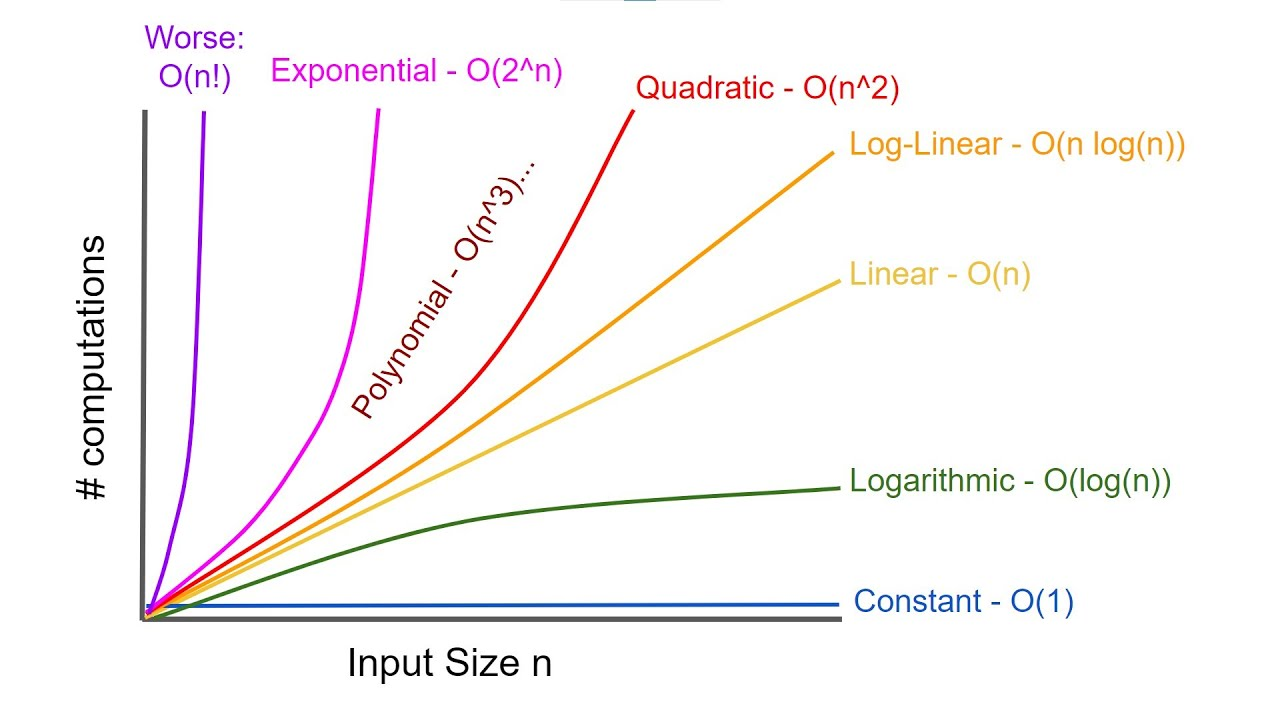
\includegraphics[scale=0.3]{timeComplexity.jpg}
    \caption{A Graphical view of Time Complexity}
    \centering
\end{figure}

The notation O in the graphic is an asymptotic notation to represent the worst-time complexity of a function, the function
inside the O is function that dominates the time complexity of a problem.
\begin{align}
f(x) &= O(g(n))
\end{align}
In the function above, the function $f$ is dominated by $g$. 
Now, we can finally enter into what is actually polynomial time. In terms of mathematical description, it can be described as
this: \[m(n) = O(n^k)\]

Where k is a constant value. It is possible to build a Deterministic Turing Machine to represent these types of functions,
which is one of the main aspects to differentiate P and NP. Since problems that have the worst time-complexity worse than the 
function above may not seem possible to be represented in a Deterministic Turing Machine, but it is known that there is a 
Non-deterministic Turing Machine that represents it, therefore, Non-deterministic polynomial (NP) time.



\subsection{P vs NP}

Following the previous section, there's a clearer way to differentiate P and NP problems, maybe solving a NP problem might be 
a huge task to solve, but to prove that the answer provided is indeed the right answer is easy, actually it's a polynomial time
problem to identify the correctness of a NP problem. For example, solving a Sudoku seems really hard, but proving that it is indeed  
correct is easy, even using a brute-force iteration, the time-complexity would just be $O(n^2)$. 

Actually we can group all P problems as NP problems. That is to say, if a problem can be solved in polynomial time, the solution of a 
problem  must be able to be verified in polynomial time, if all correct solutions have come out, verifying any given solution only 
needs to be compared. The point is, one wonders whether all NP problems are P problems. We can again use the point of view of sets 
to illustrate. If all P problems are classified into one set P, and all NP problems are classified into another set NP, then, obviously,
P belongs to NP. Now, all researches on NP problems focus on one question, whether P = NP or not? The so called "P vs NP" is actually 
just one sentence: prove or overthrow  P = NP.

The problem is still unsolved, no one has proved or overthrew this thesis, however, it is generally accepted that P = NP does not hold,  
There is a reason why people so firmly believe that P does not equal NP is that in the process of studying NP problems, a very special 
class of NP problems has been found called NP-complete problems, also known as NPC problems.

\subsection{ NP-Complete Problems}

To talk about NP-Completeness, we need to understand a few concepts. First, reducibility, basically, a problem A can 
be reduced to a problem B means that problem A can be solved with the solution of problem B, or problem A can be 
``turned into'' problem B. In the book of ``Introduction to Algorithms'' gave such an example, there are two problems: 
a linear equation and a quadratic equation. Then we say that the former can be reduced to the latter, which means that 
if you know how to solve a quadratic equation, you must be able to solve a linear equation. 

Problem A is no more difficult than problem B. It's easy to understand. Since problem A can be solved by problem B, 
if the time complexity of B is lower than that of A, then the algorithm of A can be improved to the algorithm of B, 
and the time complexity of the two is still the same. Just as solving a quadratic equation is more difficult than 
solving a linear equation, because the method for solving the former can be used to solve the latter. This concept allows
us to  go futher, because reducibility have an important property: they are transitive. If problem A can be reduced to 
problem B, and problem B can be reduced to problem C, then problem A must be reduced to problem C. 

Therefore, it is possible to say that there exists an NP problem to which all NP problems can be reduced. In other 
words, once this problem is solved, all NP problems are solved. It is unbelievable that this kind of problem exists, 
and what is even more incredible is that there is not only one such problem, there are many, and it is a kind of 
problem. This type of problem is the NP-Complete problem.

The definition of NPC-Problems is easy, first, it has to be an NP problem; then, all NP problems can be reduced to it.
And to prove a NPC-Problem is also straightforward, first, prove that it is actually an NP problem, and then prove 
that one of the known NPC problems can be reduced to it.

To look at it in another way, we can use the concept of NP-hard, a problem L is said to be NP-hard, if any NP problem 
can be polynomially reduced to L. If an NP-hard problem L itself is NP, then L is said to be NP-complete. 


\chapter{Report Body}
The central part of the report usually consists of three or four chapters detailing the technical work undertaken during the project. {\bf{\textcolor{red}{The structure of these chapters is highly project dependent}}}. They can reflect the chronological development of the project, e.g. design, implementation, experimentation, optimisation, evaluation, etc (although this is not always the best approach). However you choose to structure this part of the report, you should make it clear how you arrived at your chosen approach in preference to other alternatives. In terms of the software that you produce, you should describe and justify the design of your programs at some high level, e.g. using OMT, Z, VDL, etc., and you should document any interesting problems with, or features of, your implementation. Integration and testing are also important to discuss in some cases. You may include fragments of your source code in the main body of the report to illustrate points; the full source code is included in an appendix to your written report.

\section{Section Heading}

\subsection{Subsection Heading}
\chapter{Design \& Specification}

\section{Section Heading}
\chapter{Implementation}

\section{Section Heading}

\chapter{Legal, Social, Ethical and Professional Issues}
Your report should include a chapter with a reasoned discussion about legal, social ethical and professional issues within the context of your project problem. You should also demonstrate that you are aware of the regulations governing your project area and the Code of Conduct \& Code of Good Practice issued by the British Computer Society, and that you have applied their principles, where appropriate, as you carried out your project.

\section{Section Heading}

\chapter{Results/Evaluation}

\section{Software Testing}

\section{Section Heading}

\chapter{Conclusion and Future Work}

The project's conclusions should list the key things that have been learnt as a consequence of engaging in your project work. For example, ``The use of overloading in C++ provides a very elegant mechanism for transparent parallelisation of sequential programs'', or ``The overheads of linear-time n-body algorithms makes them computationally less efficient than $O(n \log n)$ algorithms for systems with less than 100000 particles''. Avoid tedious personal reflections like ``I learned a lot about C++ programming...'', or ``Simulating colliding galaxies can be real fun...''. It is common to finish the report by listing ways in which the project can be taken further. This might, for example, be a plan for turning a piece of software or hardware into a marketable product, or a set of ideas for possibly turning your project into an MPhil or PhD.

%%%%%%%%%%%%%%%%%%%%%%%%%%%%%%%%%
% References
%%%%%%%%%%%%%%%%%%%%%%%%%%%%%%%%%
\bibliographystyle{plain}
\bibliography{references}
\addcontentsline{toc}{section}{Bibliography}

%%%%%%%%%%%%%%%%%%%%%%%%%%%%%%%%%
% Appendices
%%%%%%%%%%%%%%%%%%%%%%%%%%%%%%%%%
\appendix
\include{Appendices/appendix}
\chapter{User Guide}
\section{Instructions}
You must provide an adequate user guide for your software. The guide should provide easily understood instructions on how to use your software. A particularly useful approach is to treat the user guide as a walk-through of a typical session, or set of sessions, which collectively display all of the features of your package. Technical details of how the package works are rarely required. Keep the guide concise and simple. The extensive use of diagrams, illustrating the package in action, can often be particularly helpful. The user guide is sometimes included as a chapter in the main body of the report, but is often better included in an appendix to the main report.

\chapter{Source Code}
\section{Instructions}
Complete source code listings must be submitted as an appendix to the report. The project source codes are usually spread out over several files/units. You should try to help the reader to navigate through your source code by providing a ``table of contents'' (titles of these files/units and one line descriptions). The first page of the program listings folder must contain the following statement certifying the work as your own: ``I verify that I am the sole author of the programs contained in this folder, except where explicitly stated to the contrary''. Your (typed) signature and the date should follow this statement.

All work on programs must stop once the code is submitted to KEATS. You are required to keep safely several copies of this version of the program and you must use one of these copies in the project examination. Your examiners may ask to see the last-modified dates of your program files, and may ask you to demonstrate that the program files you use in the project examination are identical to the program files you have uploaded to KEATS. Any attempt to demonstrate code that is not included in your submitted source listings is an attempt to cheat; any such attempt will be reported to the KCL Misconduct Committee.

\textbf{You may find it easier to firstly generate a PDF of your source code using a text editor and then merge it to the end of your report. There are many free tools available that allow you to merge PDF files.}


\end{document}
